\documentclass[a4paper]{article}

\usepackage[T2A]{fontenc}
\usepackage[utf8]{inputenc}
\usepackage[russian]{babel}


\usepackage{graphicx}
\usepackage{float}
\usepackage{mathtools}
\usepackage{wrapfig}
\usepackage{amsfonts, amssymb, amsmath, latexsym}
\usepackage{nicefrac}
\usepackage{hhline}
\usepackage{multirow}
\usepackage[colorinlistoftodos,bordercolor=orange,backgroundcolor=orange!20,linecolor=orange,textsize=scriptsize]{todonotes}
\usepackage[colorlinks=true,linkcolor=blue,citecolor=blue]{hyperref}       % hyperlinks
\usepackage{nicefrac}       % compact symbols for 1/2, etc.
\usepackage{nameref}
\usepackage{booktabs}       % professional-quality tables

\usepackage{algorithm}
\usepackage{algpseudocode}

\usepackage{xcolor, colortbl}
\usepackage{etoolbox}

% \graphicspath{ {./} }

\usepackage[verbose=true,letterpaper]{geometry}

\newgeometry{
    textheight=9in,
    textwidth=5.5in,
    top=1in,
    headheight=12pt,
    headsep=25pt,
    footskip=30pt
}

\usepackage{epigraph}

%

\newcommand{\argmin}{\mathop{\arg\!\min}}
\newcommand{\argmax}{\mathop{\arg\!\max}}

\newcommand{\Var}{\mathbb{V}}
\newcommand{\Exp}{\mathbb{E}}
\newcommand{\Cov}{\text{Cov}}
\newcommand{\makebold}[1]{\boldsymbol{#1}}
\newcommand{\mean}[1]{\overline{#1}}
\newcommand{\eps}{\varepsilon}
\renewcommand{\epsilon}{\varepsilon}

\newcommand{\partfrac}[2]{\frac{\partial #1}{\partial #2}}
\newcommand{\ttt}[1]{\texttt{#1}}
\newcommand{\term}[1]{\textbf{#1}}

\newcommand{\la}{\langle}
\newcommand{\ra}{\rangle}

\newcommand{\lp}{\left(}
\newcommand{\rp}{\right)}
\newcommand{\lf}{\left\{}
\newcommand{\rf}{\right\}}
\newcommand{\ls}{\left[}
\newcommand{\rs}{\right]}
\newcommand{\lv}{\left|}
\newcommand{\rv}{\right|}

\newcommand*{\affaddr}[1]{#1} % No op here. Customize it for different styles.
\newcommand*{\affmark}[1][*]{\textsuperscript{#1}}


\usepackage{amsthm}

\theoremstyle{definition}
\newtheorem{definition}{Определение}[section]

\newtheorem{exercise}{Задача}[section]

\newtheorem*{solution}{Решение}
\theoremstyle{remark}
\newtheorem*{remark}{Remark}

\makeatletter
\renewcommand{\l@section}{\@dottedtocline{1}{0em}{2.1em}}
\makeatother

% \setlength\epigraphwidth{.8\textwidth}
\setlength\epigraphrule{0pt}

\title{Работа 3.6.1 \\ Спектральный анализ электрических сигналов}
\author{Шарапов Денис, Б05-005}
\date{}

\usepackage{fancyhdr}
\pagestyle{fancy}
\fancyhf{}
\rhead{Работа 3.6.1}
\lhead{}
\cfoot{\thepage}
\usepackage{subcaption}
\usepackage[font={small}]{caption}

\begin{document}

    \maketitle
    \tableofcontents
    \newpage
    
\section{Аннотация}

 \textbf{Цель работы:} Изучение спектрального состава периодических электрических сигналов \\
 
 \noindent \textbf{В работе используются:} анализатор спектра, генератор прямоугольных импульсов, генератор сигналов специальной формы, осциллограф.
 
 \section{Теоретические сведения}
 
В работе изучается спектральный состав периодических электрических сигналов различной формы: последовательности прямоугольных импульсов, последовательности пугов и амплитудно-модулированных гамонических колебаний. Спектры этих сигналов наблюдаюся с помощью промышленного анализатора спектра и справниваются с рассчитанными теоретически.

 \subsection{Спектральное разложение}

 Рассмотрим функцию вида $$f(t) = \sum\limits^{N}_{n=1}A_n\cos{\omega_n t - \alpha_n},$$ где $A_n$, $\omega_n$, $\alpha_n$ --- постоянные величины. Множество пар $(\omega_1, A_1), \ldots, (\omega_n, A_n)$ называется спектром функции $f(t)$. $N$ может быть конечным или бесконечным.

\subsection{Разложение сложных сигналов на периодические колебания}

Пусть задана функция $f(t)$, которая периодически повторяется с частотой $\Omega_1 = \dfrac{2\pi}{T}$, где $T$ --- период повторения импульсов. Её разложение в ряд Фурье имеет вид 
\begin{equation}
f(t) = \dfrac{a_0}{2} + \sum\limits_{n = 1}^{\infty}\left[a_n \cos \left(n \Omega_1t\right) + b_n \sin \left(n \Omega_1t\right)\right]
\end{equation}
или
\begin{equation}
f(t) = \dfrac{a_0}{2} + \sum\limits_{n = 1}^{\infty}A_n \cos \left(n\Omega_1t-\psi_n\right).
\end{equation}
Если сигнал четен относительно $t=0$, так что $f(t) = f(-t)$ в тригонометрической записи остаются только косинусные члены. Для нечетной наоборот.

\noindent Коэффициенты определяются по формуле
\begin{equation}
\begin{array}{c}
a_n  = \dfrac{2}{T}\int\limits_{t_1}^{t_1+T}f(t)\cos\left(n \Omega_1 t\right) dt,\\
\\
b_n = \dfrac{2}{T}\int\limits_{t_1}^{t_1+T}f(t)\sin\left(n \Omega_1 t\right) dt.
\end{array}
\end{equation}
Здесь $t_1$ --- время, с которого начинается отсчет.

\noindent Сравнив формулы $(1)$ и $(2)$ можно получить выражения для $A_n$  и $\psi_n$:
\begin{equation}
A_n = \sqrt{a_n^2+b_n^2}; \quad \psi_n = \arctan \dfrac{b_n}{a_n}.
\end{equation}

\subsection{Периодическая последовательность прямоугольных импульсов}

Введем некоторые величины:
\[\Omega_1 = \dfrac{2\pi}{T}, \]
где $T$ --- период повторения импульсов.

\noindent Коэффициенты при косинусных составляющих будут равны
\begin{equation}
a_n = \dfrac{2}{T}\int\limits_{-\tau/2}^{\tau/2}V_0\cos\left(n\Omega_1 t\right)dt = 2V_0\dfrac{\tau}{T}\dfrac{\sin\left(n\Omega_1\tau/2\right)}{n\Omega_1\tau/2} \sim \dfrac{\sin x}{x}.
\end{equation}

\noindent Здесь $V_0$ - амплитуда сигнала. Поскольку функция четная, то $b_n = 0$. 

\medskip

\noindent Пусть у нас $\tau$ кратно $T$. Тогда введем ширину спектра, равную $\Delta \omega$ --- расстояние от главного максимума до первого нуля огибающей, возникающего, как нетрудно убедится при $n = \dfrac{2\pi}{\tau \Omega_1}$. При этом

\begin{equation}
\Delta \omega \tau \simeq 2\pi \Rightarrow \Delta \nu \Delta t \simeq 1.
\end{equation}

\subsection{Периодическая последовательность цугов}

Функция $f(t)$ снова является четной относительно $t = 0$. Коэффициент при $n$-ой гармонике согласно формуле $(3)$ равен

\begin{equation*}
a_n = \dfrac{2}{T}\int\limits_{-\tau/2}^{\tau/2}V_0 \cos \left(\omega_0t\right) \cdot \cos\left(n \Omega_1t\right)dt = V_0 \dfrac{\tau}{T}\left( \dfrac{\sin\left[\left(\omega_0 - n \Omega_1\right)\dfrac{\tau}{2}\right]}{\left( \omega_0 - n \Omega_1\right) \dfrac{\tau}{2}} + \dfrac{\sin\left[\left(\omega_0 + n \Omega_1\right)\dfrac{\tau}{2}\right]}{\left( \omega_0 + n \Omega_1\right) \dfrac{\tau}{2}}\right).
\end{equation*}

\subsection{Амплитудно-модулированные колебания}

Рассмотрим гармонические колебания высокой частоты $\omega_0$, амплитуда которых медленно меняется по гармоническому закону с частотой $\Omega \ll \omega_0$.

\begin{equation}
f(t) = A_0 \left[1+m\cos \Omega t\right] \cos \omega_0 t.
\end{equation}

\noindent Коэффициентом $m$ называется \textit{глубина модуляции}. При $m < 1$ амплитуда меняется от минимальной $A_{min} = A_0(1-m)$ до максимальной $A_{max} = A_0(1+m)$. Глубина модуляции может быть представлена в виде

\begin{equation}
m = \dfrac{A_{max}-A_{min}}{A_{max}+A_{min}}.
\end{equation}

\noindent С помощью тригонометрического преобразования уравнения $(8)$ можно найти спектр колебаний

\begin{equation}
f(t) = A_0 \cos \omega_0t + \dfrac{A_0m}{2} \cos \left(\omega_0 + \Omega\right)t + \dfrac{A_0m}{2}\cos\left(\omega_0 - \Omega\right)t.
\end{equation}

\newpage

\section{Результаты измерений и обработка данных}

\subsection{Исследование спектра периодической последовательности прямоугольных импульсов}

Установим прямоугольные колебания с $f_{\text{повт}} = 1$ кГц и длительностью импульса \\ $\tau =100$ мкс. Получим на экране спктр сигнала и изучим его поведение при изменении $\tau$ и $f_{\text{повт}}$. 


    \begin{center}
        \begin{tabular}{cc}
        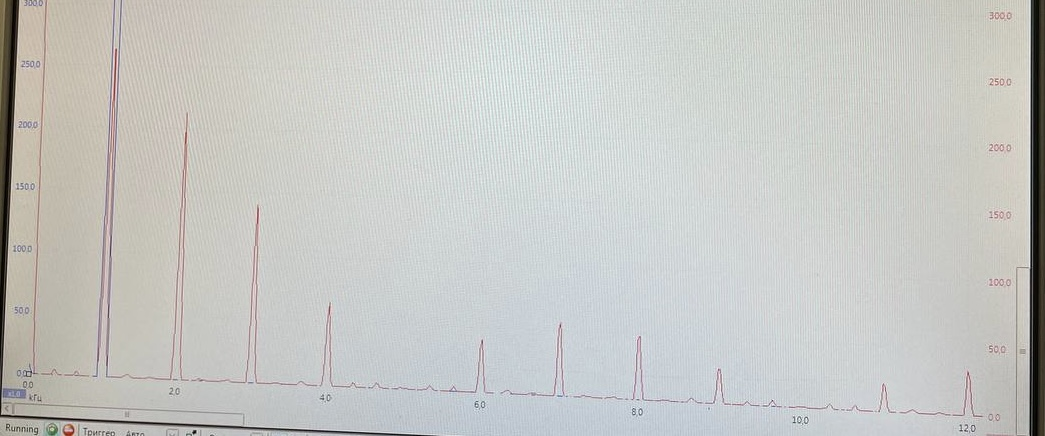
\includegraphics[width=0.45\textwidth]{image/pic1.JPG}&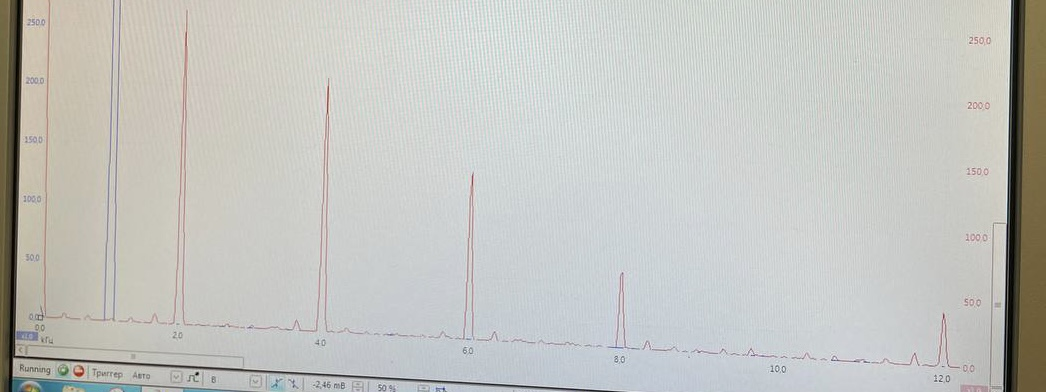
\includegraphics[width=0.45\textwidth]{image/pic2.JPG}\\
        $f_{\text{повт}} = 1$ кГц, $\tau = 100$ мкс & 
        $f_{\text{повт}} = 2$ кГц, $\tau = 100$ мкс\\
        \end{tabular}
        \end{center}

\noindent Опытным путём получаем, что при увеличении $\tau$ уменьшается $\Delta\nu$, а при увеличении $f_{\text{повт}}$ увеличивается расстояние между пиками. 

\medskip

\noindent Проведём измерения зависимости ширины спектра от длительности импульса при увеличении $\tau$ от 40 до 200 мкс при $f_{\text{повт}} = 1$ кГц. Результаты измерений внесены в таблицу~1.

\begin{table}[h!]
    \centering
    \begin{tabular}{|c|c|c|}
    \hline
    $\tau$, мкс & $\Delta\nu$, кГц & 1/$\tau$, мкс$^{-1} \cdot 10^2$ \\ \hline
    40          & 24                & 2,50                            \\ \hline
    60          & 16                & 1,67                            \\ \hline
    80          & 12                & 1,25                            \\ \hline
    100         & 9                 & 1,00                            \\ \hline
    120         & 8                 & 0,83                            \\ \hline
    140         & 6                 & 0,71                            \\ \hline
    160         & 5                 & 0,63                            \\ \hline
    180         & 4,2               & 0,56                            \\ \hline
    200         & 3,8               & 0,50                            \\ \hline
    \end{tabular}
    \caption{Результаты измерений зависимости $\Delta\nu$ от $\tau$}
    \end{table}

    \begin{figure}[h!]
        \centering
        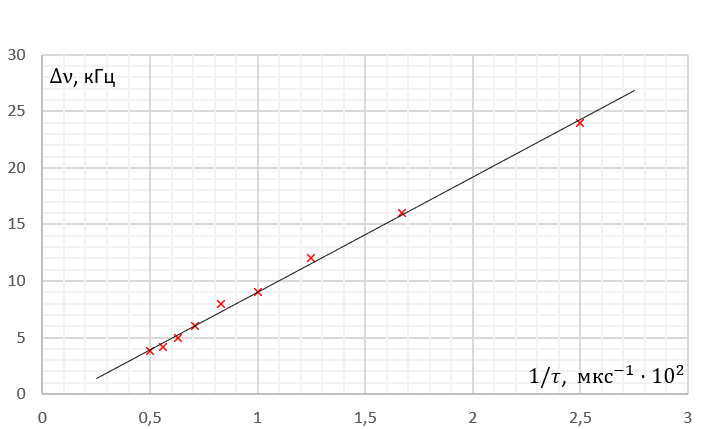
\includegraphics[width = 290pt]{image/graph1.png}
        \caption{График зависимости ширины спектра от длительности импульса}
    \end{figure}


\newpage

\subsection{Исследование спектра периодической последовательности цугов гармонических колебаний}

Проанализируем, как изменится вид спектра при увеличении длительности импульса вдвое от 100 до 200 мкс.


\begin{center}
    \begin{tabular}{cc}
    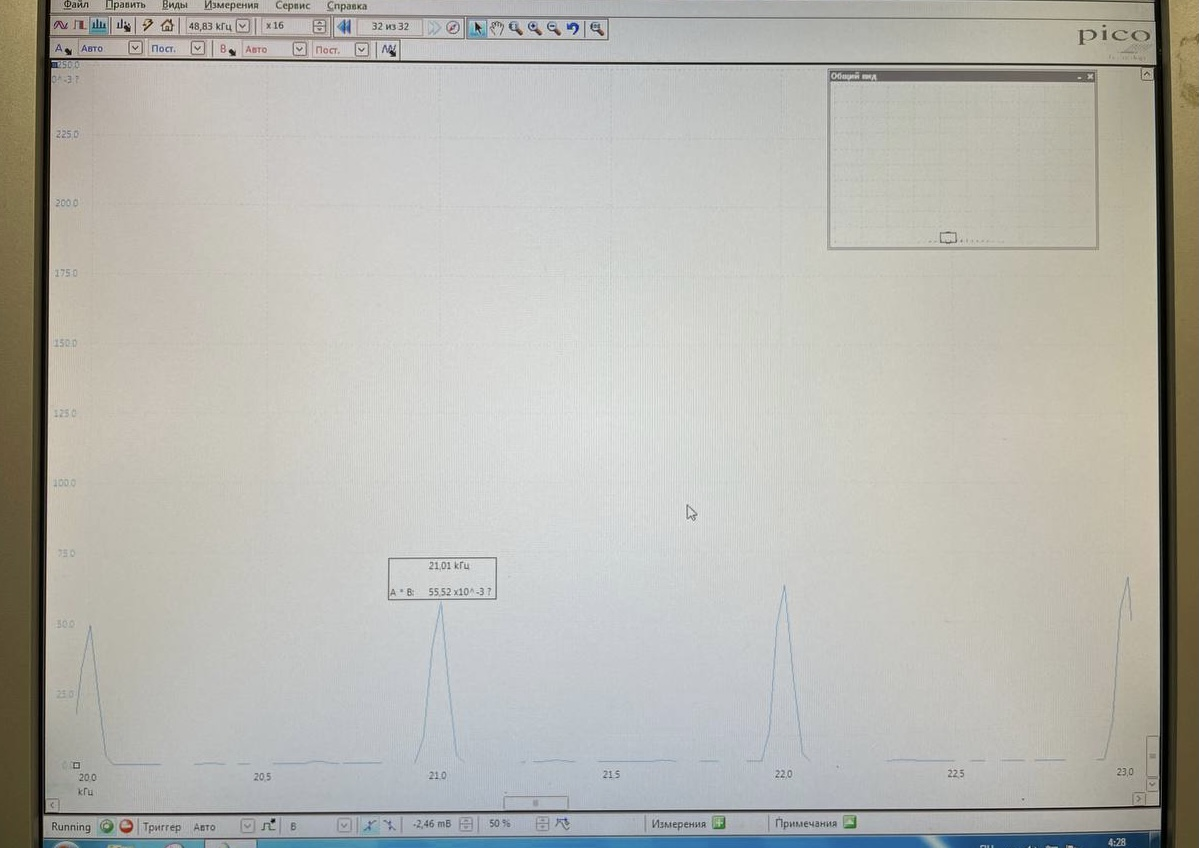
\includegraphics[width=0.45\textwidth]{image/pic100loc.JPG}&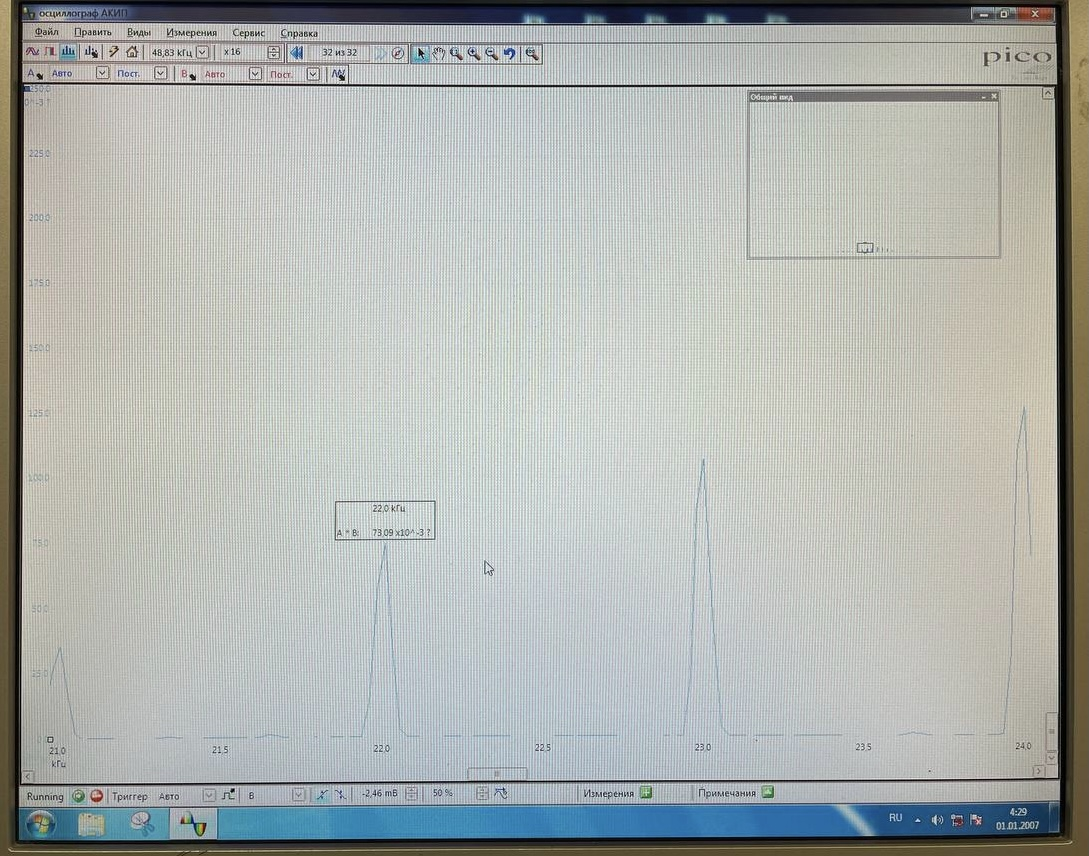
\includegraphics[width=0.45\textwidth]{image/pic200loc.JPG}\\
    $\tau = 100$ мкс, локально & 
    $\tau = 200$ мкс, локально\\
    \end{tabular}
    \end{center}

    \begin{center}
        \begin{tabular}{cc}
        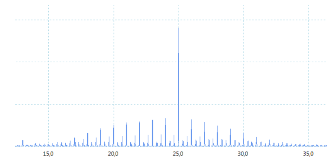
\includegraphics[width=0.45\textwidth]{image/pic100.png}&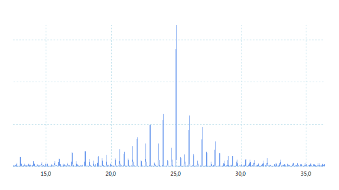
\includegraphics[width=0.45\textwidth]{image/pic200.png}\\
        $\tau = 100$ мкс, общий вид & 
        $\tau = 200$ мкс, общий вид\\
        \end{tabular}
        \end{center}

\noindent Из данных видно, что при изменении $\tau$ значение $\Delta\omega$ изменяется обратно пропорционально. \medskip

\noindent Установим длительность импулься $\tau = 100$ мкс. Проанализируем, как меняется картина спектра при изменении несущей частоты $\nu_0$.

\medskip

    \begin{center}
        \begin{tabular}{ccc}
        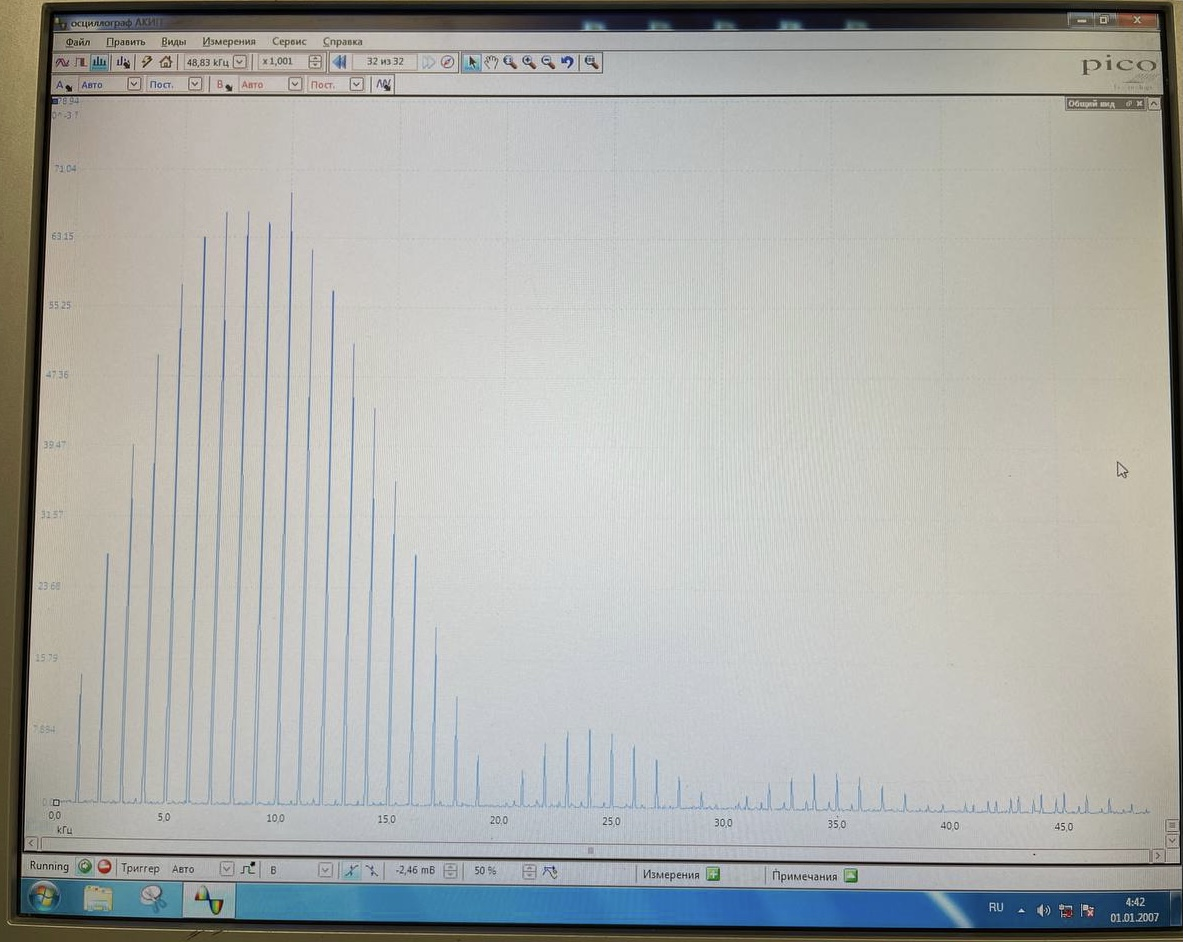
\includegraphics[width=0.30\textwidth]{image/pic10.JPG}&
        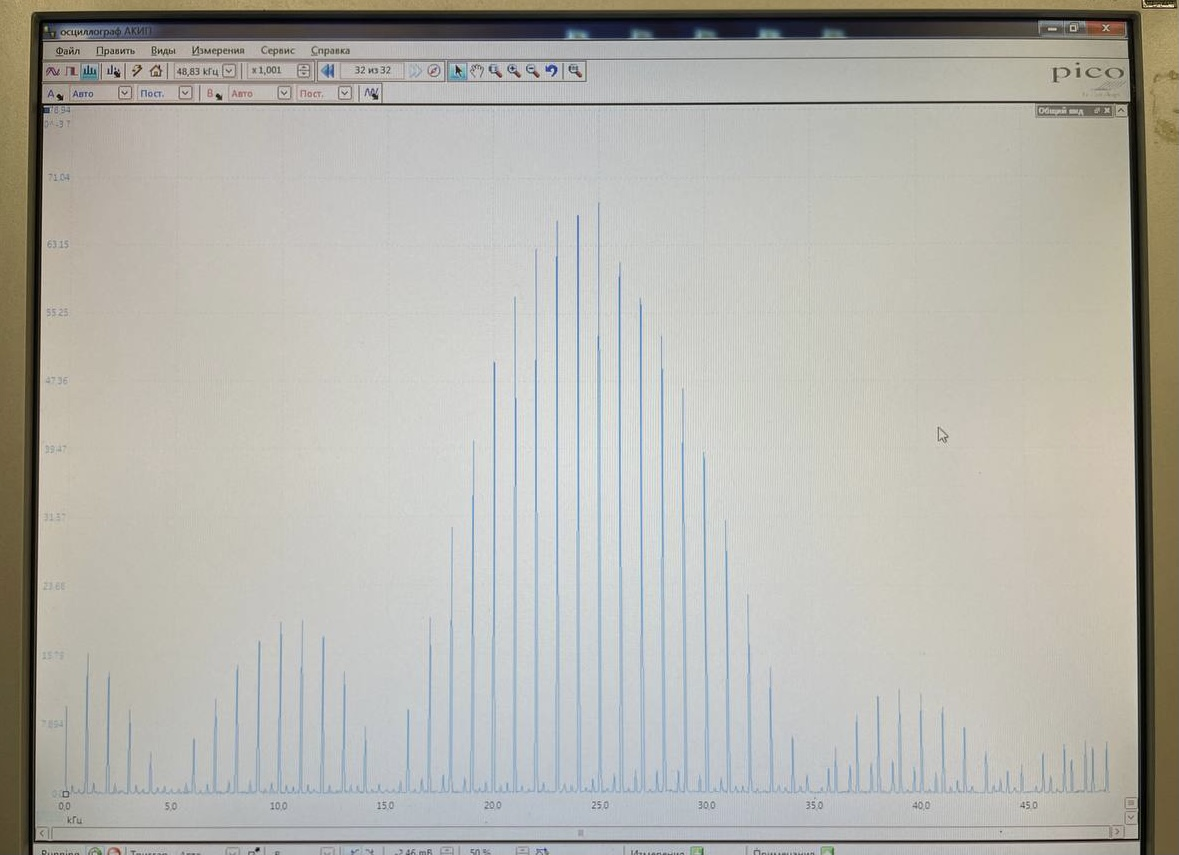
\includegraphics[width=0.30\textwidth]{image/pic25.JPG}&
        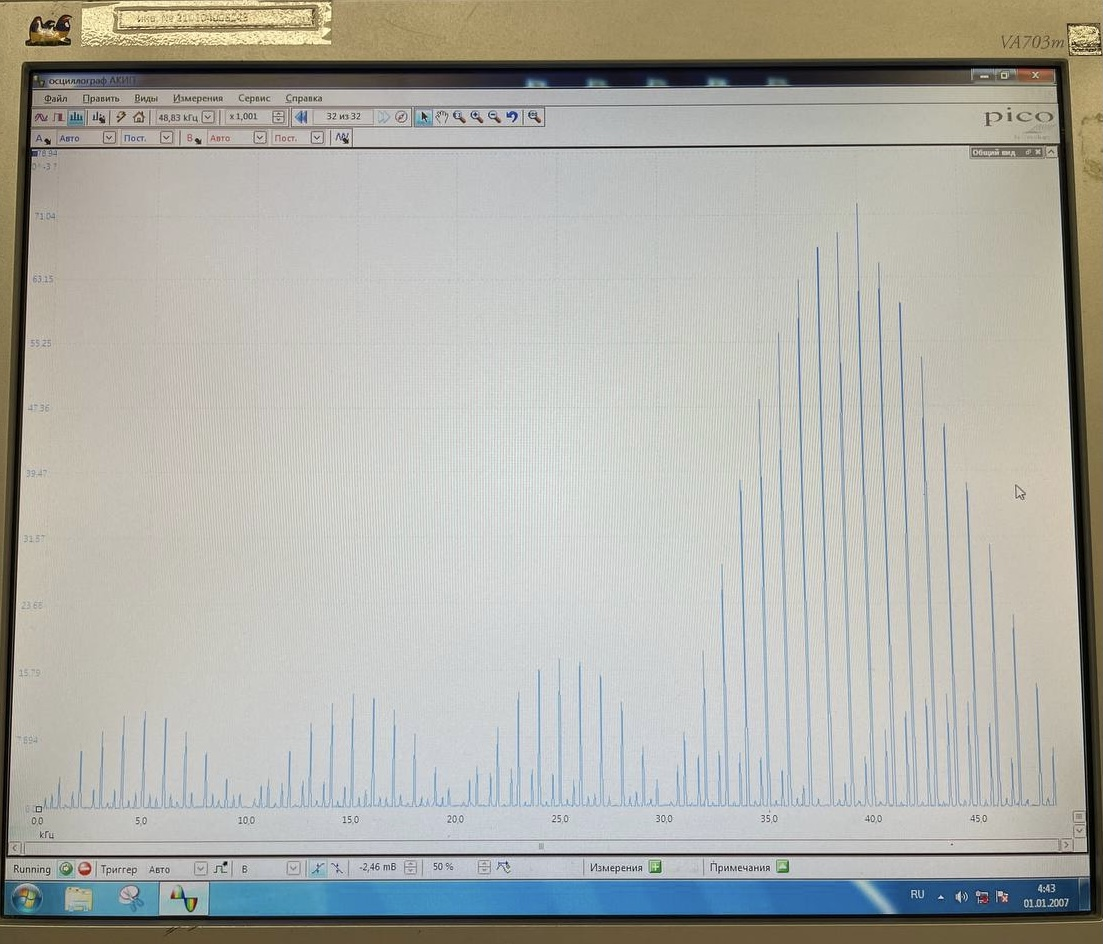
\includegraphics[width=0.30\textwidth]{image/pic40.JPG}\\
        $\nu_0 = 10$ кГц&
        $\nu_0 = 25$ кГц&
        $\nu_0 = 40$ кГц\\
        \end{tabular}
        \end{center}
        
\noindent Из данных видно, что при изменении $\nu_0$ картина смещается без изменения расстояния между спектральными компонентами.

\newpage

\noindent Определим расстояние $\delta\nu$ между соседними спектральными компонентами для разных частот повторения импульсов $f_{\text{повт}}$. Проведём измерения для $f_{\text{повт}} = 0,5, 1, 2, 4, 5$ кГц. Результаты измерений занесём в таблицу 2.

 \begin{table}[h!]
    \centering
    \begin{tabular}{|c|c|}
    \hline
    $f_{\text{повт}}$, кГц & $\delta\nu$, кГц \\ \hline
    0,5 & 0,5                \\ \hline
    1,0 & 1,0                \\ \hline
    2,0 & 2,0                \\ \hline
    4,0 & 4,0                \\ \hline
    5,0 & 5,0                \\ \hline
    \end{tabular}
    \caption{Результаты измерений $\delta\nu$}
    \end{table}


    \begin{figure}[h!]
        \centering
        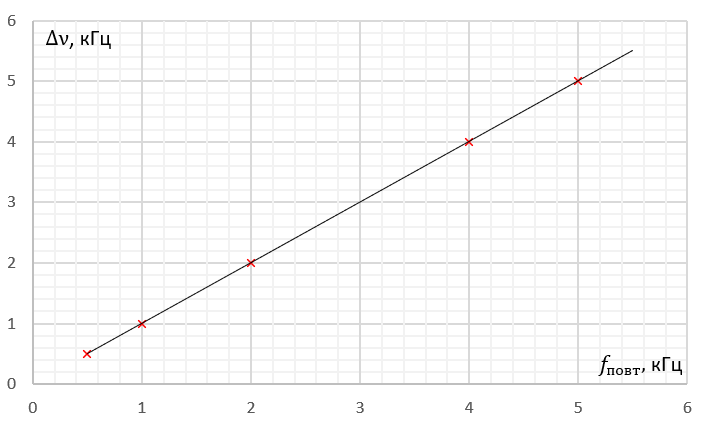
\includegraphics[width = 270pt]{image/graph2.png}
        \caption{График зависимости расстояния $\delta\nu$ от частоты повторения $f_{\text{повт}}$}
    \end{figure}


\subsection{Исследование спектра гармонических сигналов, модулированных по амплитуде.}

Меняя двойную амплитуду сигнала от 0,2 до 2 В, измерим для каждого значения максимальную $A_{max}$ и минимальную $A_{min}$ амплитуды сигналов модулированного колебания. После чего рассчитаем $m$ и $k$: $$m = \frac{A_{max} - A_{min}}{A_{max}+A_{min}},$$ $$k = \frac{A_{\text{бок}}}{A_{\text{осн}}}.$$ 

\noindent Результаты представлены в таблице 3.

\begin{table}[h!]
    \centering
    \begin{tabular}{|c|c|c|c|}
    \hline
    $(A_{max} - A_{min})$, B & $A_{\text{бок}}$, B      &  $m$   &   $k$   \\ \hline
    0,2 & 0,016 & 0,1 & 0,05 \\ \hline
    0,6 & 0,050 & 0,3 & 0,15 \\ \hline
    1,0 & 0,080 & 0,5 & 0,24 \\ \hline
    1,4 & 0,100 & 0,7 & 0,33 \\ \hline
    1,8 & 0,140 & 0,9 & 0,45 \\ \hline
    2,0 & 0,155 & 1,0 & 0,48 \\ \hline
    \end{tabular}
    \caption{Результаты измерения коэффициентов $m$ и $k$}
    \end{table}

    \begin{figure}[t]
        \centering
        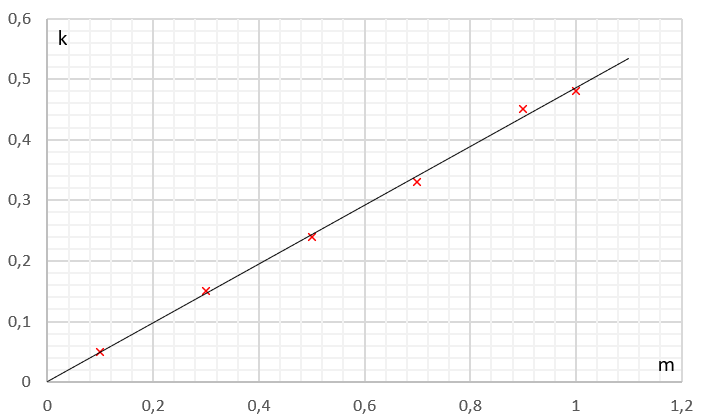
\includegraphics[width = 290pt]{image/graph3.png}
        \caption{График зависимости коээфициента $k$ от $m$}
    \end{figure}

\noindent Из МНК получим коэффициент наклона прямой $\mu$: $$\mu = \frac{k}{m} = 0,48 \pm 0,02.$$

\section{Вывод}


\end{document}